\begin{figure}[p]
\centering
\begin{tikzpicture}[x=1cm,y=1cm,
 box/.style={draw,rounded corners=2pt,align=center,inner sep=9pt,
             text width=5.7cm,minimum height=1.3cm},
 good/.style={->,very thick,draw=blue!65!black},
 zero/.style={->,very thick,draw=red!70!black}]
\node[box,fill=blue!4] (source) at (0,0)
 {$H_j(G,M_r)$\\$=\mathcal I_r\otimes\Lambda^j\mathcal V_{\rm pr}$};
\node[box,fill=blue!4] (kernel) at (8,0)
 {$H_{j-1}(G,K_r^\theta)$\\joint source kernel};
\draw[good] (source) -- node[above,align=center,font=\small]
 {$\partial^\theta_{r,j}$} node[below,font=\small] {injective} (kernel);
\node[box,fill=blue!4] (cone) at (8,-3)
 {$H_j\operatorname{Cone}(J_r\xrightarrow{E_r}I_r^A)$\\relative theta comparison};
\draw[good] (kernel) -- node[right,align=left,font=\small]
 {$\kappa_j$\\injective} (cone);
\node[box,fill=red!4] (interior) at (8,-6)
 {$H_j(G,H^{\otimes r})$\\original arithmetic interior};
\draw[zero] (cone) -- node[right,align=left,font=\small]
 {canonical map\\zero on $\kappa_j\operatorname{im}\partial^\theta_{r,j}$} (interior);
\node[align=left,text width=5.9cm,anchor=north] at (0,-1.6)
 {\textbf{Every mixed class survives.}\\[4pt]
 $\mathcal I_r$ consists of locally constant balanced-support
 functions vanishing at the $2^r$ endpoint tuples.\\[8pt]
 Count-$m$ configurations have the exact idele character
 $|a_\infty|_\infty^m\prod_p|a_p|_p^m$.\\[8pt]
 The actual cone return is $-\kappa_j\partial^\theta_{r,j}$;
 the displayed minus sign is retained.};
\node[box,fill=green!4,text width=13.9cm,anchor=north] at (4,-8)
 {\textbf{A nonzero class at every prime: $r=2$, $j=1$.}\\[8pt]
 $\displaystyle
 \begin{array}{c|ccc}
 \text{place}&\infty&p&\ell\ne p\\\hline
 \text{column on }\mathcal Z_2&(1,0)&(0,1)&(1,0)\text{ or }(0,1)
 \end{array}$\\[7pt]
 $\displaystyle
 z_p=\frac{((U_p-I)a_p)\otimes d_p}{p-1},\qquad
 [k_p]=[(U_p\otimes U_p-I)z_p]\ne0.$\\[5pt]
 Its inverse detector returns $c_p|_{\mathcal Z_2}\otimes\vartheta_p$.
 Its arithmetic return has amplitude zero, with the original support label.};
\end{tikzpicture}
\caption{Exact homology maps, with all primes retained. GSB8 gives the
domain, GSB15 the injection and entire image, GSB16 the action,
GSB21 the explicit Schwartz class, GSB21a--c its inverse detector,
and GSB22--22a the nonzero relative return with zero arithmetic
image. The third column in the table describes the restriction to
the balanced space; the original cylinder leaves those places
unrestricted. The diagram asserts no positivity of the arithmetic
pairing. Human source conventions: Connes; Connes, Consani and
Marcolli, cited in the proof.}
\end{figure}
